\chapter{Analisi delle Metodologie}


In generale un sistema che riconosce la respirazione a partire da alcuni segnali fisiologici continui, deve essere sensibile al cambiamento di alcune caratteristiche del segnale che sono omomorfe alla presenza, al volume, al flusso o alla frequenza della respirazione. 
Queste caratteristiche sono in generale dipendenti dal contesto quindi ci aspettiamo che un buon algoritmo faccia leva su delle quantit\`a statistiche del segnale o su una qualche forma di apprendimento automatico. 
Ci aspettiamo anche che tali caratteristiche rispettino un qualche principio di localit\`a questo perch\'e le propriet\`a della respirazione cambiano molto nel lungo termine.

La figura \ref{schemaGeneraleAlg} mostra uno schema generale nel quale rientrano tutti i possibili sistemi software di riconoscimento della respirazione attraverso dei sensori.
\begin{figure}[!b]
 \centering
 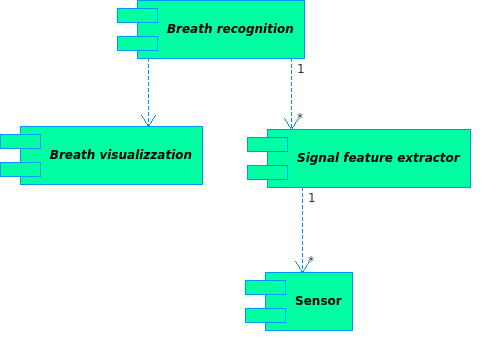
\includegraphics{./metodologiaDiagramma.png}
 % metodologiaDiagramma.png: 504x232 pixel, 96dpi, 13.33x6.14 cm, bb=0 0 378 174
  \caption{Schema generale di un software di riconoscimento della respirazione}
  \label{schemaGeneraleAlg}
\end{figure}


\section{Metodo elementare}
Siamo tentati dal dire che per risolvere il problema \`e sufficiente l'algoritmo \ref{algoritmoElementare}. 
Anche nelle ipotesi che non ci sia alcun rumore ambientale, non abbiamo la certezza che tale algoritmo funzioni per via di altri rumori fisiologici che potrebbero essere rilevati dallo stetoscopio ad esempio suoni cardiovascolari, suoni gastrointestinali e muscolari. 
L'algoritmo tuttavia \`e sottospecificato in quanto ci sono vari gradi di libert\`a: la scelta della soglia e la scelta della dimensione della finestra. 
Dai dati disponibili nella letteratura riguardo i suoni registrati da uno stetoscopio non siamo in grado di dire se possiamo scegliere i parametri dell'algoritmo in modo da farlo funzionare correttamente.
Riteniamo quindi che almeno un primo livello di trattamento del segnale sia necessario per risolvere questo problema. 
Inoltre una implementazione cos\`i banale \`e probabilmente possibile realizzarla ad un livello pi\`u basso ad esempio direttamente nel firmware dello stetoscopio. 

\incmargin{1em}
\restylealgo{boxed}\linesnumbered
\begin{algorithm}
  \dontprintsemicolon
  \SetVline
  % \SetNoline
%   \SetKwData{b}{b}
%   \SetKwData{This}{this}
%   \SetKwData{Up}{up}
  \SetKwFunction{getAverageLocalEnergy}{getAverageLocalEnergy}
  \SetKwFunction{getInstantSoundEnergy}{getSoundEnergy}
  \SetKwFunction{Write}{write}
  \SetKwFunction{Init}{init}
  \SetKwFunction{Clear}{clear}
  \SetKwFunction{Add}{add}
  \SetKwInOut{Input}{input}
  \SetKwInOut{Output}{output}
  \caption{Naive breath detection}

    \Input{A block of sound samples}
%     \Output{A boolean}
    \BlankLine
%     soundEnergyHistoryBuffer.\Clear{}\;
    \ForEach{window $w$ in the input block}{
      instantSoundEnergy $\leftarrow$ w.\getInstantSoundEnergy{}\;
%       averageLocalEnergy $\leftarrow$ soundEnergyHistoryBuffer.\getAverageLocalEnergy{}\;
%       soundEnergyHistoryBuffer.\Write{instantSoundEnergy}\;
% 			//variance = Util.getVariance(soundEnergyHistoryBuffer, averageLocalEnergy);
% 			// final double linearRegression = Util.getLinearRegression(variance);
% 			//final double linearRegression = 1;
% 			//final boolean isABeat = (instantSoundEnergy > (linearRegression * averageLocalEnergy));
      \eIf{instantSoundEnergy $>$ threshold}{
	is a breath;
% 	beatSequence.\Add{true}\;
% 	breathFrequency $\leftarrow$ (breathFrequency + 1) * (59.0 / 60.0)\;
      }{
	is not a breath;
% 	beatSequence.\Add{false}\;
% 	breathFrequency $\leftarrow$ breathFrequency * (59.0 / 60.0)\;
      }
%     \Return beatSequence\;
  }

\label{algoritmoElementare}
\end{algorithm}
\decmargin{1em}





\section{Beat detection}
La soluzione \`e nata dall'osservazione che il respiro ha un certo ritmo e quindi si pu\`o trattare il respiro come se fosse musica. 
La ricerca sul beat detection ha portato ad una serie di algoritmi e metodi per il trattamento di suoni musicali. 
Da una analisi di questi si capisce che possono essere applicati con opportune modifiche anche ai suoni prodotti dal respiro.




\subsection{Scelta dell'algoritmo}

Secondo \cite{Pekonen} ci sono varie propriet\`a da considerare per scegliere un algoritmo di onset detection. 
Ad esempio: 
\begin{itemize}
  \item
    La complessit\`a dell'algoritmo.
  \item
    Le caratteristiche della piattaforma sulla quale ci si aspetta che l'algoritmo venga usato.
  \item
    La presenza o meno di vincoli sul tempo di esecuzione dell'algoritmo. 
  \item
    Il dominio dell'input: 
    \begin{itemize}
      \item
	Se il segnale ha dei beat molto marcati e presenta relativamente poche voci(ad esempio la musica tecno) allora \`e adeguato un metodo nel dominio del tempo.
      \item
	Se il segnale da analizzare \`e complesso, ad esempio nel caso della musica sinfonica nella quale c'\`e una base di strumenti che fanno da accompagnamento e quindi dettano il ritmo della musica e altri gruppi di strumenti pi\`u legati alla melodia, allora conviene usare un metodo basato su informazione di fase nel dominio delle frequenze, in quanto in questo caso i beat sono legati molto al timbro degli strumenti.
    \end{itemize}
  \item
    Se \`e necessaria una localizzazione precisa nel tempo e nelle frequenze allora si possono usare metodi basati sulle wavelet. 
  \item
    Se la complessit\`a computazionale non \`e un problema ed \`e presente un insieme adatto di segnali di allenamento allora si possono usare metodi basati su apprendimento automatico e informazioni statistiche(reti neurali, support vector machine, modelli nascosti di Markov).
\end{itemize}

Ricordiamo che gli algoritmi di onset detection sono progettati per funzionare su brani musicali. 
Questi possono essere un insieme molto complesso di voci musicali. 
Nel nostro caso le ipotesi sull'input sono pi\`u semplici perch\'e possiamo assimilare il suono registrato dallo stetoscopio sul petto ad un brano musicale composto da due voci: i suoni respiratori e i suoni cardiovascolari. 
Anche nel caso dei suoni tracheali abbiamo due voci: i suoni respiratori e i suoni della deglutizione.
Quindi concludiamo che serve un algoritmo che sfrutta sia una analisi nel dominio delle frequenze che una analisi nel dominio del tempo.



\section{Pattern recognition e apprendimento automatico}
Un'altra possibile soluzione attinge al campo del riconoscimento vocale. 
In particolare alcune tecniche di riconoscimento vocale usano dei classificatori che hanno come mattoni di base i fonemi. 
Il suono della respirazione in un certo senso pu\`o essere pensato come un linguaggio parlato nel quale ci sono solo due tipi di fonemi: l'inspirazione e l'espirazione. 
Sia nel linguaggio parlato che nella respirazione \`e anche importante il riconoscimento del silenzio.
  
\subsection{Reti neurali}
Una soluzione di questo tipo si pu\`o implementare attraverso reti neurali. In generale si pu\`o procedere nel modo seguente:
\begin{enumerate}
  \item 
    Prima di tutto bisogna disporre di un database di registrazioni di suoni respiratori. 
  \item
    I suoni possono attraversare una fase di filtraggio nella quale si rimuove il rumore, si riduce eventualmente la frequenza di campionamento e si cerca di eliminare i suoni cardiovascolari.
  \item
    Questi suoni si segmentano in segmenti di due tipi:
    \begin{itemize}
      \item 
	Suoni che contengono respirazione, cio\`e suoni che contengono il suono prodotto dall'espirazione o dall'inspirazione
      \item
	Suoni che contengono pause respiratorie. 
	Per pause respiratorie in questo caso si intende una pausa in generale e quindi non necessariamente una apnea.
    \end{itemize}
  \item
    Per ogni segmento si calcola una sequenza di $S$ propriet\`a statistiche interessanti ad esempio: la media dei valori assoluti dei coefficienti di Fourier in determinate bande di frequenza; la potenza media dei coefficienti wavelet in determinate bande di frequenza; la deviazione standard dei coefficienti in determinate bande di frequenza; il rapporto tra la media dei valori assoluti in bande di frequenza adiacenti. 
  \item
    Si calcola inoltre la quantit\`a $l$ che \`e la media della durata dei segmenti che contengono suoni respiratori.
  \item
    A questo punto si usano i valori calcolati in precedenza per allenare una rete neurale. 
    Una rete neurale \`e un meccanismo per approssimare una funzione quindi per allenare una rete neurale bisogna fornire ad essa delle coppie $(input,\; output)$. 
    In questo caso possiamo usare due neuroni di output e un un numero di neuroni di input pari ad $n$, dove $n$ \`e il numero di propriet\`a dei segmenti di suono calcolate in precedenza. 
    Possiamo costruire un insieme di allenamento nel modo seguente. 
    Se $S$ \`e una sequenza  relativa ad un segmento di respiro allora inseriamo nell'insieme $(S, (1,0))$ mentre se $S$ \`e una sequenza relativa ad un segmento di pausa inseriamo nell'insieme $(S, (0,1))$. 
  \item	
    Dopo che la rete \`e allenata possiamo usarla per classificare un segnale di input. 
    Come prima cosa si divide il segnale in segmenti di dimensione pari ad $l$
  \item
    Si da il segmento in pasto alla rete neurale; questa produce l'output: $(s,p)$. 
  \item
    Se $s$ \`e maggiore di $p$ allora il segmento \`e un suono; altrimenti \`e una pausa.
\end{enumerate}


\section{Clustering}
% DBSCAN nel quale la distanza tra due punti aumenta con la distanza temporale e diminuisce con il quadrato della y
\label{clusteringMetodologia}

Guardando il grafico della forma d'onda del segnale della respirazione, in assenza di forte rumore, nella giusta scala temporale ed entro certi limiti di quantit\`a temporale del segnale, siamo in grado di dividere il grafico in parti regolari e cicliche e di classificarle in: espirazione, inspirazione, pausa. 
Questo approccio metodologico risulta particolarmente chiaro osservando il grafico in figura \ref{grafico}.

\begin{figure}
\centering
 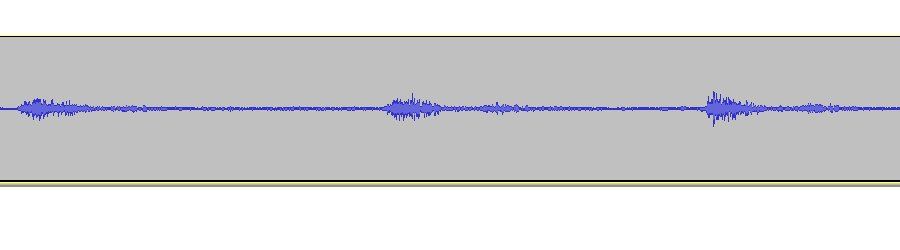
\includegraphics[width=0.7\textwidth]{./metodologiaImage.jpg}
 % metodologiaImage.xcf: 1366x768 pixel, 72dpi, 48.19x27.09 cm, bb=0 0 1366 768
  \label{grafico}
  \caption{Forma d'onda di un segnale che contiene respiro.}
\end{figure}

Tale processo intuitivo si pu\`o inquadrare nel problema pi\`u generale del clustering. Possiamo procedere nel modo seguente:
\begin{enumerate}
  \item 
    Dividere l'input in blocchi di lunghezza ad esempio $20s$ o in ogni caso un valore abbastanza grande da essere sicuri che ci sia un ciclo respiratorio completo. 
  \item
    Trovare un clustering adatto ai dati di input.
  \item
    Un respiro si pu\`o definire come un cluster di inspirazione seguito da un cluster di espirazione seguito da una pausa. Se il clustering contiene una sequenza di respiri allora il soggetto sta respirando altrimenti no.
\end{enumerate}

Rimane il problema di scegliere l'algoritmo di clustering adatto alla nostra situazione. 
Nel nostro caso siamo di fronte ad un problema di clustering nel quale lo spazio del segnale di input \`e bidimensionale. 
Una dimensione \`e il tempo discreto e l'altra dimensione \`e il valore dei campioni. 
Gli algoritmi di clustering impongono di conoscere a priori il numero di cluster oppure un valore di soglia. 
Una possibilit\`a \`e quella di usare l'algoritmo \ref{determinareClusterN} per determinare il pi\`u probabile numero di cluster. 
In seguito confrontiamo questo valore con il numero di fasi che ci dovrebbero essere in media nel blocco di input analizzato. 
Questo dovrebbe andare bene almeno per il primo blocco. 
Per i blocchi successivi possiamo tenere traccia del numero di cluster e confrontare il valore corrente con i valori passati.
